\section{Experimental Setup}{}
\label{sec:experimental_setup}

\par
The following equipment was used in the experiment:
\begin{itemize}
    \item Load Cell
    \item Instrotech Model 4004 Load Cell Interpreter
    \item FDM 3D Printer
    \item PLA and PETG filament calibrated to filament roll
    \item Test Rig
    \item Jupyter and Latex
    
\end{itemize}


\begin{figure}[H]
    \centering
        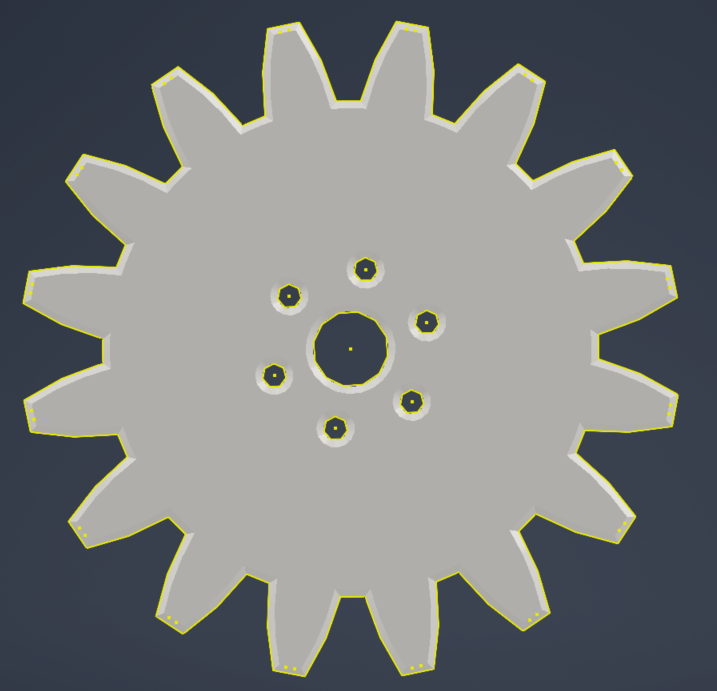
\includegraphics[width=0.75\textwidth]{img/im_gearDesignTested.png}
        \caption{Gear Design that was Tested}
        \label{im:geardesignTested}
\end{figure}

\par
A gear was designed to interface with the test rig in figure [\ref{im:testRigCAD}]. This rig uses a module 5 gear of 19mm diameter with 16 teeth and a 10mm diameter shaft hole. It has been designed with a 1mm chamfer to prevent elephant's foot while printing. It has 6 3.25mm holes for mounting screws to the flanges of the test rig. The printer has a tolerance of 0.2mm for printing in PLA and 0.3mm for PETG \cite{article_TonerPlastics}. The designed gear can be seen in figure [\ref{im:geardesignTested}].

\begin{figure}[H]
    \centering
        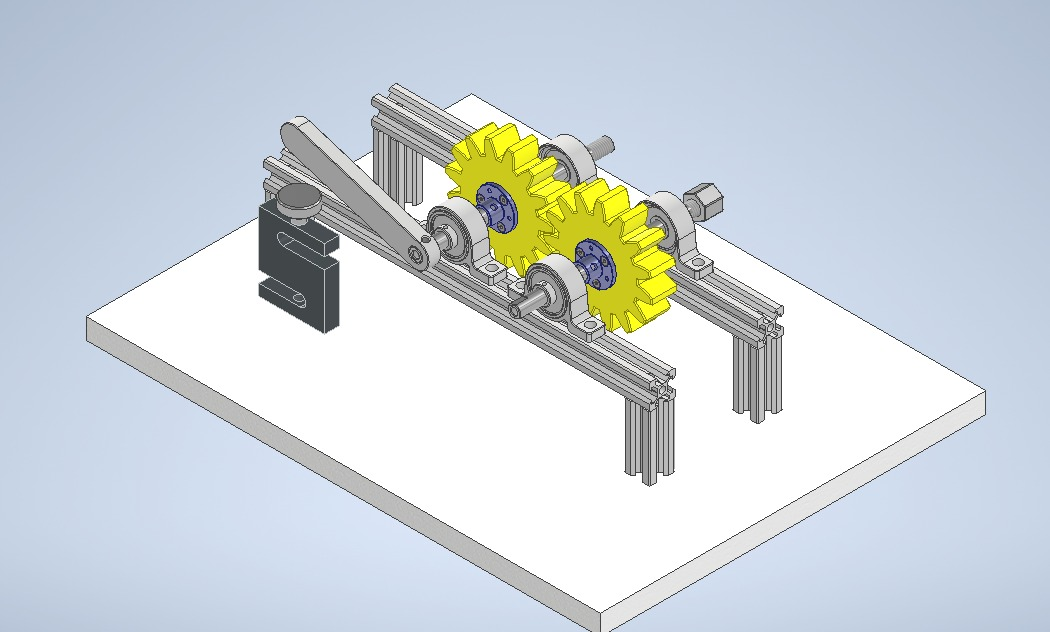
\includegraphics[width=0.75\textwidth]{img/im_testRigCAD.jpg}
        \caption{CAD Design of Rig Used to Test Gear Strength}
        \label{im:testRigCAD}
\end{figure}

\par
One gear was printed with PLA and the other with PETG. Each roll was calibrated beforehand and the relevant settings were applied. The gears were set to print with the specifications in table [\ref{tab:printsettings}]. Five layers all round are used for minimum material and maximum strength. A module five gear of this size has larger teeth than normal and if 3D printed it would have been best to print them with enough walls for solid gear teeth. This would however have increased material useage and print time with about 15 walls needed to completely fill the teeth. To compensate for this the gyroid infill setting was used to provide enough strength and general infill so that each tooth has the greatest chance of having the same strength compared to other infill settings \cite{youtube_LetsPrint}. The brim setting was used to ensure bed adhesion [\ref{im:gearSlicerSettings}]. The printed gears are shown in figure [\ref{im:2printedGears}].

\begin{table}[H]
    \centering
    \caption{Print Settings of printed gears}
    \label{tab:printsettings}
    \begin{tabular}{@{} l c @{}}
        \toprule
        \textbf{Parameter} & \textbf{Value} \\
        \midrule
        Wall Number & Value \\
        Bottom Shell Number & 5 \\
        Top Shell Number & 5 \\
        Infill Type & Gyroid \\
        Infill \% & 15 \% \\
        Brim & Outer Brim Only \\
        \bottomrule
    \end{tabular}
\end{table}

\begin{figure}[H]
    \centering
        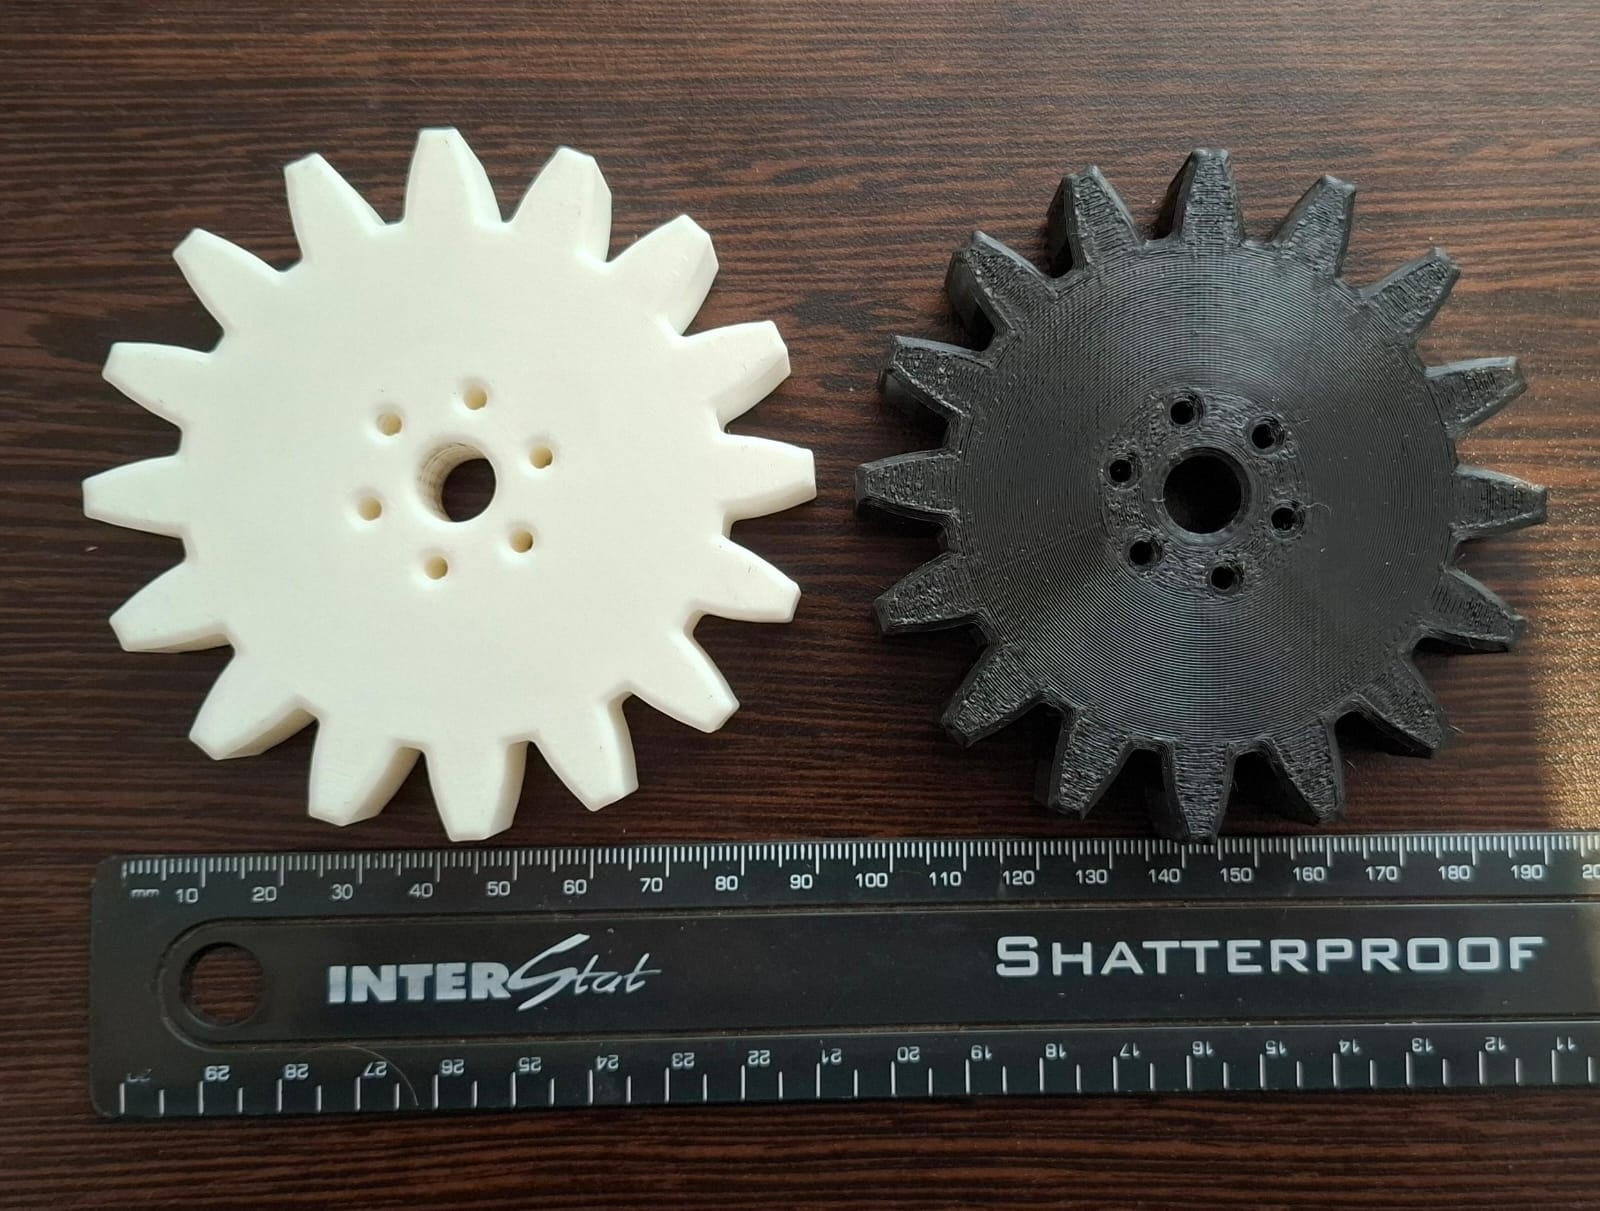
\includegraphics[width=0.75\textwidth]{img/im_2printedGears.jpeg}
        \caption{Image of the 2 Printed Gears. (White = PLA; Black = PETG)}
        \label{im:2printedGears}
\end{figure}


\begin{figure}[H]
    \centering
        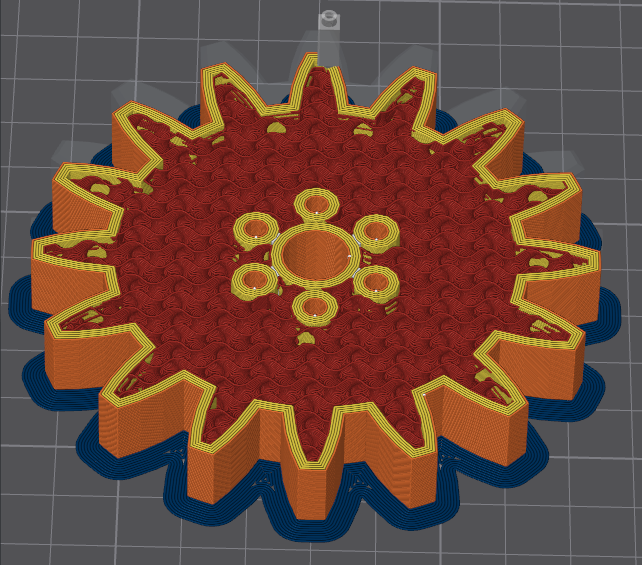
\includegraphics[width=0.75\textwidth]{img/im_gearSlicerSettings.png}
        \caption{Display of the internal slicer}
        \label{im:gearSlicerSettings}
\end{figure}


